\chapter{Topolojik Uzaylar}
\label{ch:topological_spaces}

%% ============================================================
\section{Konu}
%% ============================================================

\subsection{Sezgisel Giriş}

Topoloji, bir kümedeki noktaların birbirine ``yakın'' olup olmadığını, aralarındaki
sürekliliği ve şekilsel özellikleri, mesafe kavramına gerek duymadan inceleyen matematiksel
bir disiplindir. Bunu mümkün kılan temel araç \emph{açık küme} kavramıdır.

Düşünelim: gerçek doğruda $(a, b)$ aralığı ``açık''tır; her noktasının çevresinde küçük bir
açık aralık daha bulunur. Bu sezgiyi soyutlayarak \emph{herhangi} bir küme üzerinde topoloji
tanımlamak mümkündür.

\begin{sezgi}
Bir şehir haritasında ``yakınlık''ı sokak mesafesiyle ölçebilirsiniz; ama
``hangi mahalleler birbirine komşu?'' sorusu mesafe olmadan da anlamlıdır.
Topoloji tam bunu yapar: mesafeyi unutur, yalnızca ``hangi kümeler bir
noktanın çevresini oluşturur?'' bilgisini tutar. Matematiksel karşılığı:
$\tau$ ailesi her noktanın ``çevre'' kavramını açık kümeler aracılığıyla
kodlar; süreklilik ve yakınsama gibi kavramlar yalnız $\tau$'ya
başvurularak tanımlanır.
\end{sezgi}

\subsection{Formal Tanım}

\begin{definition}[Topolojik Uzay]
\label{def:topological_space}
Bir $X$ kümesi ve $\tau \subseteq \mathcal{P}(X)$ ailesi verilsin.
$(X, \tau)$ bir \textbf{topolojik uzay}, $\tau$ ise $X$ üzerinde bir \textbf{topoloji}
olarak adlandırılır, eğer aşağıdaki üç aksiyom sağlanıyorsa:
\begin{enumerate}
  \item[(T1)] $\emptyset \in \tau$ ve $X \in \tau$
  \item[(T2)] $U, V \in \tau \Rightarrow U \cap V \in \tau$
  \item[(T3)] $\{U_\alpha\}_{\alpha \in I} \subseteq \tau \Rightarrow
              \displaystyle\bigcup_{\alpha \in I} U_\alpha \in \tau$
\end{enumerate}
$\tau$'nun elemanları \textbf{açık küme} olarak adlandırılır.
\end{definition}

Aksiyomların her biri ayrı bir iş görür: (T1) uzayın tamamının ve boş
kümenin her zaman ``gözlemlenebilir'' olmasını garanti eder; (T2) iki
gözlemin kesişiminin de gözlem olmasını sağlar --- sonlu kesişimle sınırlı
kalması bilinçli bir tercihtir (bkz.\ Teorem~\ref{thm:axiom_sufficiency});
(T3) keyfî birleşime izin vererek küçük çevrelerden büyük çevre kurma
işlemini serbest bırakır.

\begin{karsiornek}
$X=\{1,2,3\}$ üzerinde $\sigma=\{\emptyset,\{1\},\{2\},X\}$ ailesi bir
topoloji \emph{değildir}: $\{1\}\cup\{2\}=\{1,2\}\notin\sigma$
olduğundan (T3) ihlal edilir. (T1) ve (T2) sağlansa bile tek bir eksik
birleşim aileyi topoloji olmaktan çıkarır. Bu ailenin
\texttt{make\_topology}'ye verilince ne olduğunu Örnekler bölümündeki
``Dikkat'' kutusunda göreceğiz.
\end{karsiornek}

\subsection{Temel Örnekler}

\begin{table}[h]
\centering
\begin{tabular}{lll}
\toprule
\textbf{Topoloji} & \textbf{Tanım} & \textbf{Açık kümeler} \\
\midrule
Ayrık (discrete) & Her alt küme açık & $\tau = \mathcal{P}(X)$ \\
İndirgenmiş (indiscrete) & Yalnızca $\emptyset$ ve $X$ açık & $\tau = \{\emptyset, X\}$ \\
Kosonlu (cofinite) & $U$ açık $\iff$ $U=\emptyset$ veya $X\setminus U$ sonlu & — \\
Sierpiński & $X=\{0,1\}$, $\tau = \{\emptyset, \{1\}, X\}$ & 3 açık küme \\
\bottomrule
\end{tabular}
\caption{Standart topoloji örnekleri}
\end{table}

\subsection{Baz ve Alt-Baz}

\begin{definition}[Baz]
\label{def:basis}
$\mathcal{B} \subseteq \tau$ ailesi, her $U \in \tau$ ve her $x \in U$ için
$x \in B \subseteq U$ sağlayan bir $B \in \mathcal{B}$ varsa $\tau$'ya \textbf{baz} denir.
\end{definition}

Şekil~\ref{fig:ch04:baz} koşulu resmeder: açık kümenin her noktası,
tamamen o kümenin içinde kalan bir baz elemanıyla sarılır.

\begin{figure}[ht]
  \centering
  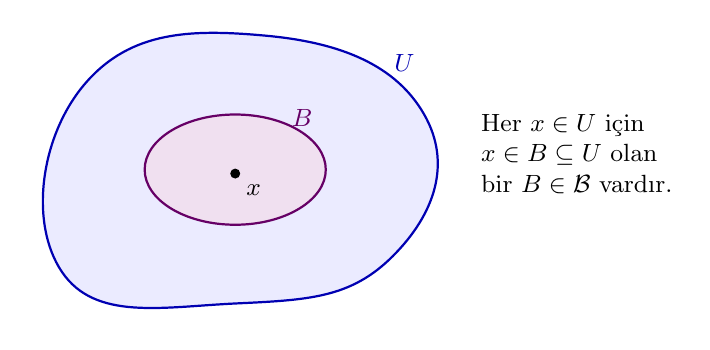
\begin{tikzpicture}[scale=1.0, font=\small]
  \draw[blue!70!black, thick, fill=blue!8]
    plot[smooth cycle, tension=0.8] coordinates
    {(0,0) (2.2,-0.4) (4.2,0.2) (4.6,2.0) (2.6,3.0) (0.3,2.4)};
  \node[blue!70!black] at (4.35,2.65) {$U$};
  \draw[violet!80!black, thick, fill=violet!12]
    (2.2,1.3) ellipse [x radius=1.15, y radius=0.7];
  \node[violet!80!black] at (3.05,1.95) {$B$};
  \fill (2.2,1.25) circle (1.8pt) node[below right=0.5pt] {$x$};
  \node[align=left, anchor=west] at (5.2,1.5)
    {Her $x\in U$ için\\ $x\in B\subseteq U$ olan\\ bir $B\in\mathcal{B}$ vardır.};
\end{tikzpicture}

  \caption{Baz koşulunun geometrisi: $U$ açık kümesinin her $x$ noktası
    için $x\in B\subseteq U$ sağlayan bir $B\in\mathcal{B}$ vardır.
    Topolojinin tüm açıkları bu tür ``yapı taşları''nın birleşimleridir.}
  \label{fig:ch04:baz}
\end{figure}

\begin{nedenonemli}
Baz, büyük bir topolojiyi küçük bir çekirdekle temsil etme aracıdır.
Gerçek doğrunun standart topolojisi sayılamaz çoklukta açık küme içerir;
ama tümü, sayılabilir $\{(a,b): a<b,\ a,b\in\mathbb{Q}\}$ bazından
üretilir. \texttt{pytop} tarafında \texttt{topology\_from\_basis} tam bu
ilkeyle çalışır: yalnız baz elemanlarını verirsiniz, kapanışı kütüphane
hesaplar (Algoritma~\ref{alg:basis_to_topology}).
\end{nedenonemli}

\noindent\textbf{Baz Koşulları:}
\begin{enumerate}
  \item[(B1)] $\bigcup \mathcal{B} = X$
  \item[(B2)] $B_1, B_2 \in \mathcal{B}$ ve $x \in B_1 \cap B_2$ ise bir $B_3 \in \mathcal{B}$
              vardır: $x \in B_3 \subseteq B_1 \cap B_2$
\end{enumerate}

\begin{definition}[Alt-Baz]
$\mathcal{S} \subseteq \mathcal{P}(X)$ ailesi; sonlu kesişimleri baz, onların birleşimleri
ise $\tau$'yu oluşturur.
\end{definition}

\subsection{Sonlu ve Sonsuz Uzaylar}

\texttt{pytop}'ta iki temel sınıf bulunur:
\begin{itemize}
  \item \textbf{\texttt{FiniteTopologicalSpace}:} Taşıyıcı $(X)$ sonlu; topoloji açıkça
        \texttt{frozenset}'ler koleksiyonu olarak saklanır. Tüm hesaplamalar tam ve kesindir.
  \item \textbf{Sonsuz türevler:} Taşıyıcı simgesel (\texttt{'R'}, \texttt{'N'});
        \texttt{topology=None}; etiket tabanlı sembolik çıkarım yapılır.
\end{itemize}

%% ============================================================
\section{Teoremler}
%% ============================================================

\begin{theorem}[Aksiyomların Yeterliliği]
\label{thm:axiom_sufficiency}
$(X, \tau)$ bir topolojik uzay olsun. T1--T3 aksiyomları, sonlu herhangi bir açık küme
ailesinin kesişiminin $\tau$'da yer aldığını garanti eder:
\[
  U_1, \ldots, U_n \in \tau \Rightarrow \bigcap_{i=1}^{n} U_i \in \tau.
\]
\textit{Not:} Sonsuz kesişim gerekmez. Gerçek doğruda
$\bigcap_{n=1}^{\infty}\bigl(-\tfrac{1}{n}, \tfrac{1}{n}\bigr) = \{0\}$
açık değildir.
\end{theorem}

\begin{proof}[Rehberli Kanıt]
\textbf{Strateji:} $n$ üzerinde tümevarım; tek araç (T2).
\begin{enumerate}
  \item $n=1$: $U_1\in\tau$ zaten verili.
  \item $n=k$ için doğru varsayalım: $V=\bigcap_{i=1}^{k}U_i\in\tau$.
  \item $n=k+1$: $\bigcap_{i=1}^{k+1}U_i = V\cap U_{k+1}$ olup (T2)
        gereği $\tau$'dadır.
\end{enumerate}
Sonsuz kesişimde 3.~adım çalışmaz: tümevarım yalnız sonlu $n$'lere
ulaşır. Şekil~\ref{fig:ch04:kesisim} bunun gerçek bir başarısızlık
olduğunu gösterir: her sonlu kesişim açıkken limit $\{0\}$ açık değildir.
\end{proof}

\begin{figure}[ht]
  \centering
  \begin{tikzpicture}[font=\small, xscale=2.8]
  \draw[-{Stealth}] (-1.35,0) -- (1.5,0) node[right] {$\mathbb{R}$};
  \draw (-1,0.05) -- (-1,-0.05) node[below, font=\scriptsize] {$-1$};
  \draw (0,0.05) -- (0,-0.05);
  \draw (1,0.05) -- (1,-0.05) node[below, font=\scriptsize] {$1$};
  \draw[blue!75, very thick] (-1,0.85) -- (1,0.85);
  \node[blue!75, font=\scriptsize, right] at (1.04,0.85) {$(-1,1)$};
  \draw[blue!55, very thick] (-0.5,0.62) -- (0.5,0.62);
  \node[blue!55, font=\scriptsize, right] at (1.04,0.62) {$(-\tfrac12,\tfrac12)$};
  \draw[blue!40, very thick] (-0.25,0.39) -- (0.25,0.39);
  \node[blue!40, font=\scriptsize, right] at (1.04,0.39) {$(-\tfrac14,\tfrac14)$};
  \node at (0,0.22) {$\vdots$};
  \fill[red!70!black] (0,0) circle (1.2pt);
  \node[red!70!black, below=7pt, font=\scriptsize] at (0,-0.02)
    {$\bigcap_n \bigl(-\tfrac1n,\tfrac1n\bigr)=\{0\}$ --- açık değil};
\end{tikzpicture}

  \caption{(T2)'nin sonlu kesişimle sınırlı olmasının nedeni: iç içe
    $(-\tfrac1n,\tfrac1n)$ açık aralıklarının sonsuz kesişimi tek
    noktaya çöker ve $\{0\}$ standart topolojide açık değildir.}
  \label{fig:ch04:kesisim}
\end{figure}

\begin{theorem}[Baz Teoremi]
\label{thm:basis}
$\mathcal{B} \subseteq \mathcal{P}(X)$ ailesi \emph{(B1)--(B2)} koşullarını sağlıyorsa,
\[
  \tau_{\mathcal{B}}
  = \bigl\{U \subseteq X : \forall x \in U,\, \exists B \in \mathcal{B},\,
    x \in B \subseteq U\bigr\}
\]
bir topoloji olur ve $\mathcal{B}$ bu topolojiye baz oluşturur.
\end{theorem}

\begin{proof}[Rehberli Kanıt]
\textbf{Strateji:} $\tau_{\mathcal{B}}$'nin üç aksiyomu sağladığını, her
adımda yalnız (B1)--(B2)'yi kullanarak doğrularız.
\begin{enumerate}
  \item \textbf{(T1):} $\emptyset\in\tau_{\mathcal B}$, çünkü ``her
        $x\in\emptyset$ için\ldots'' koşulu boş yere doğrudur.
        $X\in\tau_{\mathcal B}$: $x\in X$ verilsin; (B1) gereği
        $x\in\bigcup\mathcal B$, yani $x\in B\subseteq X$ olan bir
        $B\in\mathcal B$ vardır.
  \item \textbf{(T2):} $U,V\in\tau_{\mathcal B}$ ve $x\in U\cap V$
        olsun. Tanım gereği $x\in B_U\subseteq U$ ve
        $x\in B_V\subseteq V$ bulunur. (B2), $x\in B_3\subseteq
        B_U\cap B_V\subseteq U\cap V$ veren bir $B_3$ sağlar; $x$
        keyfî olduğundan $U\cap V\in\tau_{\mathcal B}$.
  \item \textbf{(T3):} $x\in\bigcup_\alpha U_\alpha$ ise
        $x\in U_{\alpha_0}$ olan bir indis vardır; $U_{\alpha_0}$'ın
        tanımından gelen $B$, $x\in B\subseteq
        U_{\alpha_0}\subseteq\bigcup_\alpha U_\alpha$ koşulunu da sağlar.
  \item $\mathcal B$'nin $\tau_{\mathcal B}$'ye baz olması,
        $\tau_{\mathcal B}$'nin tanımının Tanım~\ref{def:basis}'teki
        koşulu birebir içermesindendir.
\end{enumerate}
\end{proof}

\noindent Bu teorem, \texttt{topology\_from\_basis}'in döndürdüğü
ailenin gerçekten topoloji olduğunun matematiksel güvencesidir;
fonksiyon ayrıca (B1)--(B2)'yi sağlamayan girdiyi
\texttt{BasisConstructionError} ile reddeder.

\begin{theorem}[Karşılaştırma]
\label{thm:comparison}
$X$ üzerinde iki topoloji $\tau_1 \subseteq \tau_2$ ise $\tau_1$ \textbf{kaba (coarser)},
$\tau_2$ \textbf{ince (finer)} topoloji olarak adlandırılır. Ayrık topoloji en ince,
indirgenmiş topoloji en kaba topolojidir.
\end{theorem}

\begin{proof}[Rehberli Kanıt]
Herhangi bir $\tau$ için $\tau\subseteq\mathcal{P}(X)=\tau_{\mathrm{disc}}$
topoloji tanımının kendisinden gelir (aksiyom gerekmez); (T1) aksiyomu da
$\{\emptyset,X\}=\tau_{\mathrm{ind}}\subseteq\tau$ verir.
\end{proof}

\begin{figure}[ht]
  \centering
  \begin{tikzpicture}[font=\small,
    kutu/.style={draw, rounded corners, align=center, inner sep=8pt}]
  \node[kutu, fill=orange!6] (kaba) at (0,0)
    {$\tau_{\mathrm{ind}}$ (kaba)\\[3pt] $\emptyset,\quad \{a,b\}$};
  \node[kutu, fill=blue!6] (ince) at (6.4,0)
    {$\tau_{\mathrm{disc}}$ (ince)\\[3pt] $\emptyset,\ \{a\},\ \{b\},\ \{a,b\}$};
  \draw[-{Stealth[length=3mm]}, thick]
    (kaba) -- node[above] {$\subseteq$} node[below] {açık küme eklenir} (ince);
\end{tikzpicture}

  \caption{Aynı $X=\{a,b\}$ üzerinde iki uç: indirgenmiş topoloji (kaba)
    ile ayrık topoloji (ince). Açık küme eklemek topolojiyi inceltir;
    tüm topolojiler bu iki uç arasında yaşar.}
  \label{fig:ch04:kabaince}
\end{figure}

\noindent\texttt{pytop} bu uçları \texttt{tags} ile işaretler:
\texttt{indiscrete\_topology} nesnesi \texttt{indiscrete},
\texttt{discrete\_topology} nesnesi \texttt{discrete} etiketi taşır.

%% ============================================================
\section{Algoritmalar}
%% ============================================================

\subsection{Bazdan Topoloji Üretimi}

\textbf{Problem:} $X$ ve $\mathcal{B} \subseteq \mathcal{P}(X)$ verilsin;
$\tau_{\mathcal{B}}$'yi hesapla.

\begin{algorithm}
\caption{Bazdan Topoloji Üretimi}
\label{alg:basis_to_topology}
\begin{algorithmic}[1]
\Require $X$ (taşıyıcı), $\mathcal{B}$ (baz ailesi)
\Ensure $\tau$ (kapalı topoloji)
\State $\tau \leftarrow \{\emptyset, X\}$
\For{each non-empty $\mathcal{S} \subseteq \mathcal{B}$}
    \State $\tau.\text{add}\bigl(\bigcup_{B \in \mathcal{S}} B\bigr)$
\EndFor
\State \Call{CloseUnderIntersection}{$\tau$}
\Return $\tau$
\end{algorithmic}
\end{algorithm}

\begin{algorithm}
\caption{Kesişim Altında Kapatma}
\begin{algorithmic}[1]
\State $\textit{changed} \leftarrow \textbf{true}$
\While{$\textit{changed}$}
    \State $\textit{changed} \leftarrow \textbf{false}$
    \For{each $U, V \in \tau$}
        \If{$U \cap V \notin \tau$}
            \State $\tau.\text{add}(U \cap V)$;\quad $\textit{changed} \leftarrow \textbf{true}$
        \EndIf
    \EndFor
\EndWhile
\end{algorithmic}
\end{algorithm}

\noindent\textbf{Karmaşıklık:}
\begin{itemize}
  \item En kötü durum: $O(|\mathcal{B}| \cdot 2^{|\mathcal{B}|})$
        (tüm alt-ailelerin birleşimi)
  \item Pratik (çakışmayan baz elemanları): $O(|\tau| \cdot |\mathcal{B}|)$
  \item Uzay: $O(|\tau|)$ açık küme saklar
\end{itemize}

\subsection{İz Sürme: Küçük Bir Girdiyle Adım Adım}

$X=\{1,2,3\}$, $\mathcal{B}=\{\{1\},\{2,3\}\}$ girdisiyle
Algoritma~\ref{alg:basis_to_topology}:

\begin{table}[ht]
\centering
\begin{tabular}{clll}
\toprule
\textbf{Adım} & $\mathcal{S}$ (alt-aile) & \textbf{Eklenen birleşim} & $\tau$ \textbf{(o ana dek)} \\
\midrule
0 & --- & --- & $\{\emptyset, X\}$ \\
1 & $\{\{1\}\}$ & $\{1\}$ & $\{\emptyset, X, \{1\}\}$ \\
2 & $\{\{2,3\}\}$ & $\{2,3\}$ & $\{\emptyset, X, \{1\}, \{2,3\}\}$ \\
3 & $\{\{1\},\{2,3\}\}$ & $\{1\}\cup\{2,3\}=X$ & değişmez \\
4 & kesişim kapanışı & $\{1\}\cap\{2,3\}=\emptyset$ & değişmez \\
\bottomrule
\end{tabular}
\caption{İz sürme: $|\tau|=4$; döngü yeni küme üretmeyince durur.}
\end{table}

\subsection{Alt-Bazdan Topoloji Üretimi}

$\mathcal{S}$ verilsin; önce $\mathcal{S}$'nin sonlu kesişimlerinden baz oluştur,
ardından Algoritma~\ref{alg:basis_to_topology}'yi uygula.

\noindent\textbf{Karmaşıklık:} $O(|\mathcal{S}|^k \cdot 2^{|\mathcal{S}|^k})$ —
$k$: kesişim derinliği.

%% ============================================================
\section{pytop API}
%% ============================================================

\subsection{Sınıflar}

\begin{lstlisting}[language=Python, caption={Temel sınıf importları}]
from pytop import TopologicalSpace, FiniteTopologicalSpace
\end{lstlisting}

\begin{table}[h]
\centering
\begin{tabular}{lll}
\toprule
\textbf{Sınıf} & \textbf{Taşıyıcı} & \textbf{Topoloji} \\
\midrule
\texttt{TopologicalSpace} & \texttt{Any} & \texttt{Any} (None olabilir) \\
\texttt{FiniteTopologicalSpace} & sonlu \texttt{frozenset} & \texttt{frozenset[frozenset]} \\
\bottomrule
\end{tabular}
\caption{Temel uzay sınıfları}
\end{table}

\noindent\textbf{Alanlar:} \texttt{carrier} (altta yatan küme), \texttt{topology}
(açık kümeler), \texttt{tags} (özellik etiketleri), \texttt{metadata} (ek bilgiler).

\subsection{Oluşturucular}

\begin{lstlisting}[language=Python, caption={Topoloji oluşturucu importları}]
from pytop import (
    make_topology, discrete_topology, indiscrete_topology,
    cofinite_topology, sierpinski_space,
    topology_from_basis, topology_from_subbasis,
)
\end{lstlisting}

\begin{table}[h]
\centering
\begin{tabular}{lll}
\toprule
\textbf{Fonksiyon} & \textbf{İmza} & \textbf{Açıklama} \\
\midrule
\texttt{make\_topology} & \texttt{(carrier, *open\_sets)} & Açık küme listesiyle inşa \\
\texttt{discrete\_topology} & \texttt{(*elements)} & Ayrık topoloji \\
\texttt{indiscrete\_topology} & \texttt{(*elements)} & İndirgenmiş topoloji \\
\texttt{cofinite\_topology} & \texttt{(*elements)} & Kosonlu topoloji \\
\texttt{sierpinski\_space} & \texttt{()} & Sierpiński uzayı \\
\texttt{topology\_from\_basis} & \texttt{(carrier, basis)} & Bazdan topoloji üret \\
\texttt{topology\_from\_subbasis} & \texttt{(carrier, subbasis)} & Alt-bazdan topoloji üret \\
\bottomrule
\end{tabular}
\caption{Topoloji oluşturucu fonksiyonlar}
\end{table}

\subsection{Tag Sistemi}

\texttt{pytop} nesneleri \texttt{tags} kümesi aracılığıyla topolojik özellikler taşır.
Örnek etiketler: \texttt{"finite"}, \texttt{"discrete"}, \texttt{"t0"}, \texttt{"t1"},
\texttt{"hausdorff"}, \texttt{"compact"}, \texttt{"connected"}, \texttt{"metric"}.

\subsection{Tag Gerekçeleri}

Etiketler, kurucunun inşa anında \emph{garanti ettiği} gerçeklerdir:

\begin{table}[ht]
\centering
\begin{tabular}{lp{4.2cm}p{5.6cm}}
\toprule
\textbf{Kurucu} & \textbf{Etiketler} & \textbf{Gerekçe} \\
\midrule
\texttt{sierpinski\_space()} & compact, connected, finite, t0 &
  Sonlu $\Rightarrow$ kompakt; $\{1\}$ tek yönlü ayırır $\Rightarrow$ T0
  (T1 değil); ayrık parçalanış yok $\Rightarrow$ bağlantılı \\
\texttt{discrete\_topology(1,2,3)} & discrete, finite, hausdorff,
  metrizable, normal, regular &
  Her tekil açık $\Rightarrow$ tüm ayrılma aksiyomları; 0--1 metriği
  ayrık topolojiyi üretir \\
\texttt{indiscrete\_topology(1,2,3)} & compact, connected, finite,
  indiscrete & Açık yalnız $\emptyset$ ve $X$: parçalanamaz \\
\texttt{cofinite\_topology('a','b','c')} & cofinite, compact, finite,
  t1 & Tekiller kapalı $\Rightarrow$ T1 \\
\texttt{make\_topology(\ldots)},
  \texttt{finite\_chain\_space(n)} & finite &
  Özellik çıkarımı yapılmaz; yalnız sonluluk işaretlenir \\
\bottomrule
\end{tabular}
\caption{Pilot bölümdeki kurucuların etiket gerekçeleri}
\end{table}

\noindent Etiketler \emph{eksiksiz değildir}:
\texttt{cofinite\_topology('a','b','c')} aslında ayrıktır ve
Hausdorff'tur ($2^3=8$ açık), ama \texttt{discrete}/\texttt{hausdorff}
etiketi taşımaz --- \texttt{is\_t2} yüklemi yine \texttt{true} döner.
Kesin sorgu için Bölüm~\ref{ch:separation}'daki \texttt{is\_*}
yüklemlerini kullanın; etiket, yüklemin yerine geçmez.

%% ============================================================
\section{Örnekler}
%% ============================================================

\subsection{Örnek 1: Sierpiński Uzayı}

\begin{lstlisting}[language=Python, caption={Sierpiński uzayı}]
from pytop import sierpinski_space

s = sierpinski_space()
print("Tasiyici:", s.carrier)
print("Topoloji:", sorted(str(t) for t in s.topology))
print("Etiketler:", sorted(s.tags))
\end{lstlisting}

\begin{lstlisting}[caption={Çıktı}]
Tasiyici: frozenset({0, 1})
Topoloji: ['frozenset()', 'frozenset({0, 1})', 'frozenset({1})']
Etiketler: ['compact', 'connected', 'finite', 't0']
\end{lstlisting}

\paragraph{Ne oldu?}
Çıktıdaki üç satırı tek tek okuyalım. \texttt{Tasiyici} satırı
$X=\{0,1\}$'i verir. \texttt{Topoloji} satırındaki üç küme tam olarak
Tanım~\ref{def:topological_space}'in istediği yapıdır: $\emptyset$ ve
$X$ (T1), tek ek açık küme $\{1\}$; $\{1\}\cap X=\{1\}$ ve
$\{1\}\cup X=X$ zaten listede olduğundan (T2)--(T3) de sağlanır.
\texttt{Etiketler} satırında \texttt{t0} var ama \texttt{t1} yok:
$1$'i içerip $0$'ı dışlayan açık küme vardır ($\{1\}$), fakat $0$'ı
içerip $1$'i dışlayan açık küme yoktur --- T0 sağlanıp T1'in
sağlanmamasının kaynağı budur (Bölüm~\ref{ch:separation}, Örnek~1'de
yüklemlerle test edilir). Şekil~\ref{fig:ch04:sierpinski} açık küme
yapısını gösterir.

\begin{figure}[ht]
  \centering
  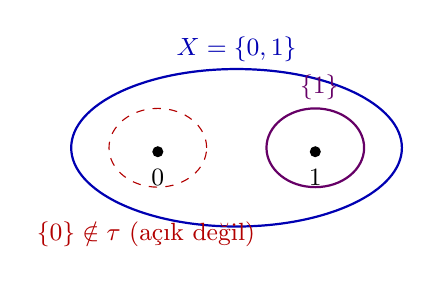
\begin{tikzpicture}[font=\small]
  \fill (0,0) circle (2pt) node[below=3pt] {$0$};
  \fill (2,0) circle (2pt) node[below=3pt] {$1$};
  \draw[blue!70!black, thick] (1,0.05) ellipse [x radius=2.1, y radius=1.0];
  \node[blue!70!black] at (1,1.3) {$X=\{0,1\}$};
  \draw[violet!80!black, thick] (2,0.05) ellipse [x radius=0.62, y radius=0.5];
  \node[violet!80!black] at (2.05,0.82) {$\{1\}$};
  \draw[red!70!black, dashed] (0,0.05) ellipse [x radius=0.62, y radius=0.5];
  \node[red!70!black] at (-0.15,-1.05) {$\{0\}\notin\tau$ (açık değil)};
\end{tikzpicture}

  \caption{Sierpiński uzayının açıkları: $\emptyset$, $\{1\}$ ve $X$.
    Kesikli bölge $\{0\}$'ın açık \emph{olmadığını} vurgular; bu
    asimetri uzayı T0 yapar ama T1 yapmaz.}
  \label{fig:ch04:sierpinski}
\end{figure}

\subsection{Örnek 2: Ayrık Topoloji}

\begin{lstlisting}[language=Python, caption={Ayrık topoloji}]
from pytop import discrete_topology

d = discrete_topology(1, 2, 3)
print("|tau| =", len(d.topology))
print("Etiketler:", sorted(d.tags))
\end{lstlisting}

\begin{lstlisting}[caption={Çıktı}]
|tau| = 8
Etiketler: ['discrete', 'finite', 'hausdorff', 'metrizable', 'normal', 'regular']
\end{lstlisting}

\paragraph{Ne oldu?}
$n=3$ eleman için $|\tau|=2^3=8$: her alt küme açıktır. Her tekil küme
açık olduğundan herhangi iki nokta kendi tekil komşuluklarıyla ayrılır
--- \texttt{hausdorff}, \texttt{normal}, \texttt{regular} etiketlerinin
kaynağı budur. \texttt{metrizable}, 0--1 metriğinden gelir:
$d(x,y)=1$ $(x\neq y)$ metriği tam olarak ayrık topolojiyi üretir.
Listede \texttt{compact} yok; oysa uzay sonlu olduğu için kompakttır ve
\texttt{is\_compact} yüklemi \texttt{true} döner --- fark için Tag
Gerekçeleri tablosuna bakın.

\subsection{Örnek 3: \texttt{make\_topology} ile Manuel İnşa}

\begin{lstlisting}[language=Python, caption={Manuel topoloji inşası}]
from pytop import make_topology

sp = make_topology({1, 2, 3}, {1}, {2, 3})
print("|tau| =", len(sp.topology))
print("Acik kumeler:", sorted(str(t) for t in sp.topology))
\end{lstlisting}

\begin{lstlisting}[caption={Çıktı}]
|tau| = 4
Acik kumeler: ['frozenset()', 'frozenset({1, 2, 3})',
               'frozenset({1})', 'frozenset({2, 3})']
\end{lstlisting}

\paragraph{Ne oldu?}
\texttt{make\_topology} verilen $\{1\}$ ve $\{2,3\}$ açıklarına yalnızca
$\emptyset$ ve $X$'i ekledi; $|\tau|=4$. Bu örnekte sonuç geçerli bir
topolojidir, çünkü verilen iki küme ayrıktır: birleşimleri $X$,
kesişimleri $\emptyset$ zaten ailededir. \texttt{make\_topology} bu
kapanışları \emph{hesaplamaz} --- aşağıdaki kutu, kapalı olmayan bir
aile verildiğinde ne olduğunu gösterir.

\begin{dikkat}
\texttt{make\_topology} verdiğiniz aileye yalnızca $\emptyset$ ve $X$'i
ekler; birleşim/kesişim kapanışını \textbf{hesaplamaz} ve aksiyomları
\textbf{denetlemez}. Aşağıdaki çağrıda $\{1\}\cup\{2\}=\{1,2\}$ ailede
yoktur; dönen nesne (T3)'ü ihlal eden, geçersiz bir ``topoloji''dir.
Kapanışın hesaplanmasını ve ailenin denetlenmesini istiyorsanız
\texttt{topology\_from\_basis} kullanın --- o, baz koşullarını
sağlamayan aileyi \texttt{BasisConstructionError} ile reddeder.
\end{dikkat}

\begin{lstlisting}[language=Python, caption={Kapanış hesaplanmaz --- sorumluluk kullanıcıda}]
from pytop import make_topology, topology_from_basis

sessiz = make_topology({1, 2, 3}, {1}, {2})   # denetlemez!
print("make_topology:", sorted(sorted(t) for t in sessiz.topology))

try:
    topology_from_basis({1, 2, 3}, [{1}, {2}])  # B1 ihlali
except Exception as e:
    print("topology_from_basis:", type(e).__name__)
\end{lstlisting}

\begin{lstlisting}[style=output, caption={Çıktı}]
make_topology: [[], [1], [1, 2, 3], [2]]
topology_from_topology: BasisConstructionError
\end{lstlisting}

\subsection{Örnek 4: Alexandrov Zincir Uzayı}

\begin{lstlisting}[language=Python, caption={Zincir uzayı}]
from pytop import finite_chain_space

c = finite_chain_space(3)
print("Tasiyici:", c.carrier)
print("Topoloji:", sorted(str(t) for t in c.topology))
\end{lstlisting}

\begin{lstlisting}[caption={Çıktı}]
Tasiyici: (1, 2, 3)
Topoloji: ['set()', '{1, 2, 3}', '{1, 2}', '{1}']
\end{lstlisting}

\paragraph{Ne oldu?}
Çıktıdaki açıklar tam bir ``önek merdiveni''dir:
$\emptyset\subset\{1\}\subset\{1,2\}\subset\{1,2,3\}$. Alexandrov zincir
uzayında $1$ her boş olmayan açıkta yer alır (``en açık'' nokta), $3$
yalnız $X$'te görünür. Öneklerin kesişimi ve birleşimi yine önek
olduğundan (T2)--(T3) otomatik sağlanır.

\subsection{Örnek 5: Bazdan Topoloji Üretimi}

\begin{lstlisting}[language=Python, caption={Bazdan topoloji}]
from pytop import topology_from_basis

b = [{1}, {2, 3}, {4}]
ts = topology_from_basis({1, 2, 3, 4}, b)
print("Baz:", [set(x) for x in b])
print("|tau| =", len(ts.topology))
print("Topoloji:", sorted(str(t) for t in ts.topology))
\end{lstlisting}

\begin{lstlisting}[caption={Çıktı}]
Baz: [{1}, {2, 3}, {4}]
|tau| = 8
Topoloji: ['set()', '{1, 2, 3, 4}', '{1, 2, 3}', '{1, 4}',
           '{1}', '{2, 3, 4}', '{2, 3}', '{4}']
\end{lstlisting}

\paragraph{Ne oldu?}
Baz $\{\{1\},\{2,3\},\{4\}\}$ bir bölüntüdür: elemanları ikişer ikişer
ayrıktır. (B2) koşulu boş yere sağlanır (kesişimler boş olduğundan
kontrol edilecek nokta yoktur) ve topoloji tüm alt-aile
birleşimlerinden oluşur: $2^3=8$ açık küme. Çıktıdaki 8 küme, üç baz
elemanının $2^3$ alt kümesinin birleşimleriyle birebir eşleşir.

\subsection{Örnek 6: Gerçek Doğru}

\begin{lstlisting}[language=Python, caption={Gerçek doğru}]
from pytop import real_line_metric

rl = real_line_metric()
print("Tasiyici:", rl.carrier)
print("Etiketler:", sorted(rl.tags))
\end{lstlisting}

\begin{lstlisting}[caption={Çıktı}]
Tasiyici: R
Etiketler: ['complete', 'connected', 'first_countable', 'hausdorff',
            'infinite', 'lindelof', 'metric', 'not_compact',
            'path_connected', 'second_countable', 'separable', 't0', 't1', 'uncountable']
\end{lstlisting}

\paragraph{Ne oldu?}
\texttt{Tasiyici: R} satırı taşıyıcının \emph{simgesel} olduğunu söyler:
gerçek doğrunun noktaları bellekte tutulmaz, \texttt{topology=None}'dır.
Tüm topolojik bilgi etiketlerde kodlanmıştır: \texttt{connected},
\texttt{hausdorff}, \texttt{second\_countable} gibi olumlu özellikler
yanında \texttt{not\_compact} gibi olumsuz bilgi de taşınır
(Heine--Borel: $\mathbb{R}$ sınırlı değildir). Sonlu uzaylardaki
``hesapla ve doğrula'' yaklaşımının yerini burada ``bilinen teoremleri
etiketle'' yaklaşımı alır; metrik tarafı Bölüm~14'te derinleşir.

%% ============================================================
\section{Alıştırmalar}
%% ============================================================

\subsection*{Kodlama Alıştırmaları}

\begin{enumerate}[label=\textbf{K\arabic*.}]
  \item \label{ex:ch04:K1} \texttt{cofinite\_topology('a','b','c')} ile üç
        noktalı kosonlu uzayı kurun; topolojisini ve etiketlerini
        yazdırın, \texttt{is\_t1} ve \texttt{is\_t2} ile test edin.
        Gözlem: sonlu bir kümede kosonlu topoloji ayrık topolojiyle
        çakışır. T1 olup Hausdorff olmayan bir örnek için taşıyıcının
        neden sonsuz olması gerektiğini bir cümleyle açıklayın
        (krş.\ Bölüm~\ref{ch:separation}, Örnek~2).
        \ipucu{$|\tau|=2^3$ çıkacak; anahtar, Bölüm~\ref{ch:separation}'daki
        ``Sonlu T1 $\iff$ Ayrık'' teoremidir.}
        (\hyperref[sol:ch04:K1]{çözüm})

  \item \label{ex:ch04:K2} \texttt{topology\_from\_subbasis(\{1,2,3,4\},
        [\{1,2\},\{3,4\},\{2,3\}])} çağrısının ürettiği topolojinin kaç
        açık küme içerdiğini bulun ve açık kümeleri listeleyin.
        \ipucu{Önce alt-baz çiftlerinin kesişimlerini elle listeleyin
        ($\{2\}$, $\{3\}$, $\emptyset$); sonra birleşimleri sayın.}
        (\hyperref[sol:ch04:K2]{çözüm})

  \item \label{ex:ch04:K3} \texttt{finite\_chain\_space(5)} ile bir
        Alexandrov-5 zinciri oluşturun; topolojinin kaç açık küme
        içerdiğini ve hangi elemanın ``en açık'' nokta olduğunu bulun.
        \ipucu{Açıklar önek yapısındadır; ``en açık'' nokta her boş
        olmayan açıkta bulunandır.}
        (\hyperref[sol:ch04:K3]{çözüm})
\end{enumerate}

\subsection*{Teori Alıştırmaları}

\begin{enumerate}[label=\textbf{T\arabic*.}]
  \item \label{ex:ch04:T1} $X=\{1,2,3\}$ üzerinde kaç farklı topoloji
        tanımlanabilir? Bu sayıyı T1--T3 aksiyomlarını doğrudan kontrol
        ederek hesaplamak yerine neden baz teoremini kullanmak daha
        pratiktir?
        \ipucu{Aday aile sayısı $2^{2^3}=256$'dır; cevap 29. Baz teoremi
        adayları üretken küçük ailelere indirger.}
        (\hyperref[sol:ch04:T1]{çözüm})

  \item \label{ex:ch04:T2} Ayrık topolojinin her zaman diğer
        topolojilerden daha ince, indirgenmiş topolojinin ise daha kaba
        olduğunu kanıtlayın. Kanıt için T1--T3 aksiyomlarından hangisi
        gereklidir?
        \ipucu{Ayrıklık için aksiyom gerekmez
        ($\tau\subseteq\mathcal{P}(X)$ tanım gereğidir); indirgenmişlik
        için yalnız (T1) yeter.}
        (\hyperref[sol:ch04:T2]{çözüm})
\end{enumerate}
